\section{Simulación }

En esta parte de la memoria presentamos el funcionamiento de la simulación, basada en un método de Monte-Carlo, tal y como especificamos a continuación. Nosotros vamos a simular la reacción de trasferencia $^{11}\text{Li}(d,t)^{10}\text{Li}$, aunque en el experimento se medirán de forma simultánea las reacciones $^{11}\text{Li}(d,p)^{12}\text{Li}$ y  $^{11}\text{Li}(d,d)^{11}\text{Li}$, cada una con un objetivo diferente. 

El algoritmo de simulación se detalla a continuación, para cada uno de sus pasos:
\begin{enumerate}

    \item  Debido a la naturaleza de estado no ligado del $^{10}$Li este aparece como una resonancia, por lo que manera intrínseca la energía de excitación del núcleo sigue una distribución de Breit-Wigner, que tendremos que tener en cuenta.
    
    La \textbf{distribución de Breit-Wigner}, es una función utilizada para modelar la distribución en energía de estados resonantes inestables. Representa la probabilidad de encontrar un sistema con una energía cercana a la energía central de la resonancia $E_{ex}$, con un ancho $\Gamma$ que caracteriza su vida media $\tau$ ($\Gamma \propto 1/\tau$). La forma de la distribución refleja el hecho de que las resonancias tienen una anchura finita en energía debido al principio de incertidumbre.
    
    La ecuación de la distribución de Breit-Wigner $g(E)$ es:
    \begin{equation}
        g(E) = \frac{A \cdot  \Gamma^2}{(E - E_{ex})^2 + \Gamma^2/4},
    \end{equation}
    donde $E$ es la energía, $E_{ex}$ la energía central de la resonancia, $\Gamma$ el ancho de la misma, y $A$ es un factor de normalización.
     
    Así pues, con cada interacción generaremos a partir de la energía resonante media $E_{ex}$ y la anchura de la resonancia $\Gamma(E_{ex})$ un valor aleatorio que siga dicha distribución, como se puede ver en \cref{Fig:04-Ex0} y \cref{Fig:04-Ex2}.
    
    \begin{minipage}{0.49\linewidth} \centering
        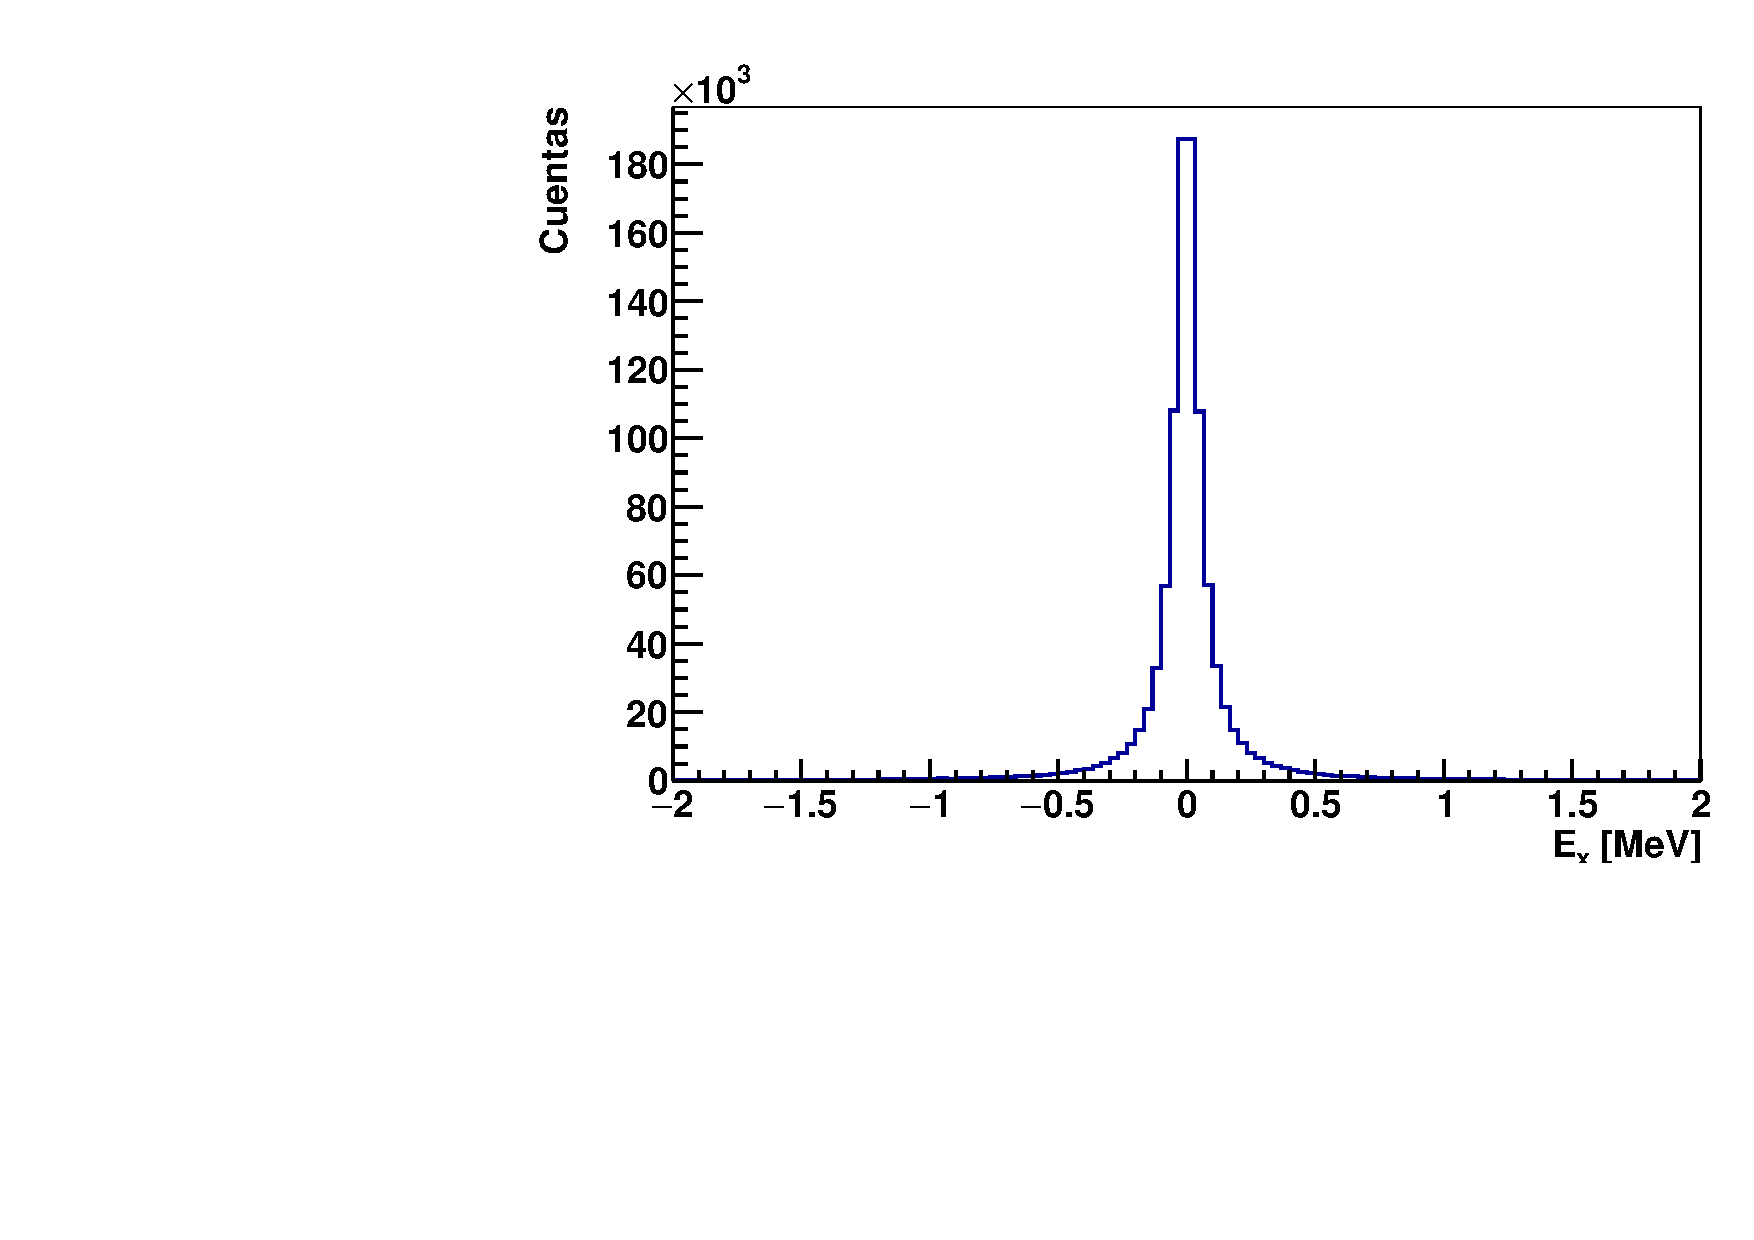
\includegraphics[width=1.0\linewidth]{Imagenes/ExHisto/ExSampled_Ex0.00_incIdx0.pdf} 
        \captionof{figure}{Distribución de las energías de excitación sampleadas $E^*=0.0$ MeV y $\Gamma=0.1$ MeV.}

        \label{Fig:04-Ex0}
    \end{minipage} \hfill
    \begin{minipage}{0.49\linewidth}
        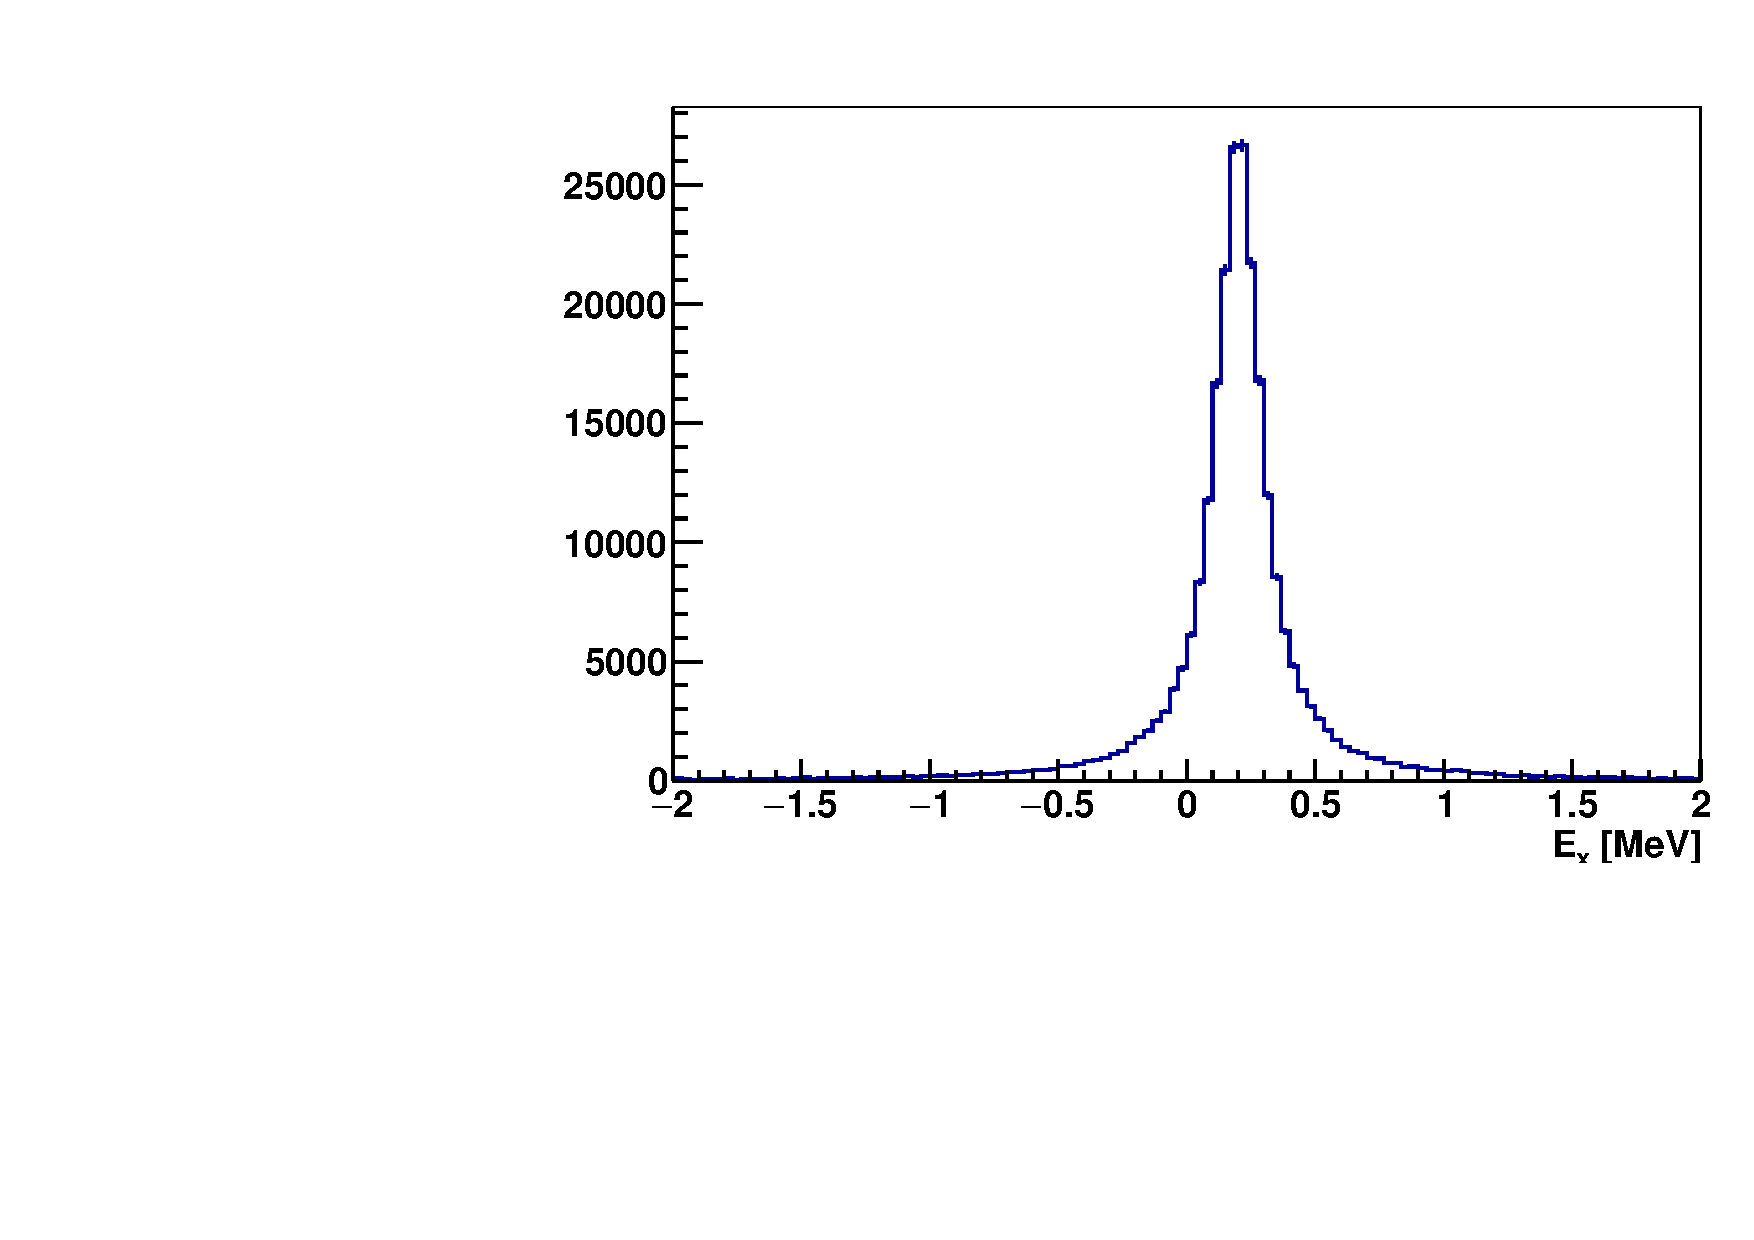
\includegraphics[width=1.0\linewidth]{Imagenes/ExHisto/ExSampled_Ex0.20_incIdx0.pdf} 
        \captionof{figure}{Distribución de las energías de excitación sampleadas $E^*=0.2$ MeV y $\Gamma=0.2$ MeV.}

        \label{Fig:04-Ex2}
    \end{minipage}
    
    

    \item  Suponemos que el haz incidente tiene una energía de $7.5$ MeV/A, que interacciona en un punto aleatorio a lo largo de la dirección del haz con una dirección $\hnx$. El punto de interacción se elige de forma aleatoria, con una distribución uniforme a lo largo del eje $X$ a lo largo de la dimensión de la cámara de deriva, mientras que en los ejes $Z$ e $Y$ se eligen a través de una distribución gaussiana centrada en el centro de la cámara de deriva con $\sigma= 3$ mm, tal y como mostramos en \cref{Fig:04-Vertex}. Estos valores están basados en los valores típicos de los haces que encontramos en el TRIUMF, Canadá, donde se realizará el experimento.  


    \begin{center}
        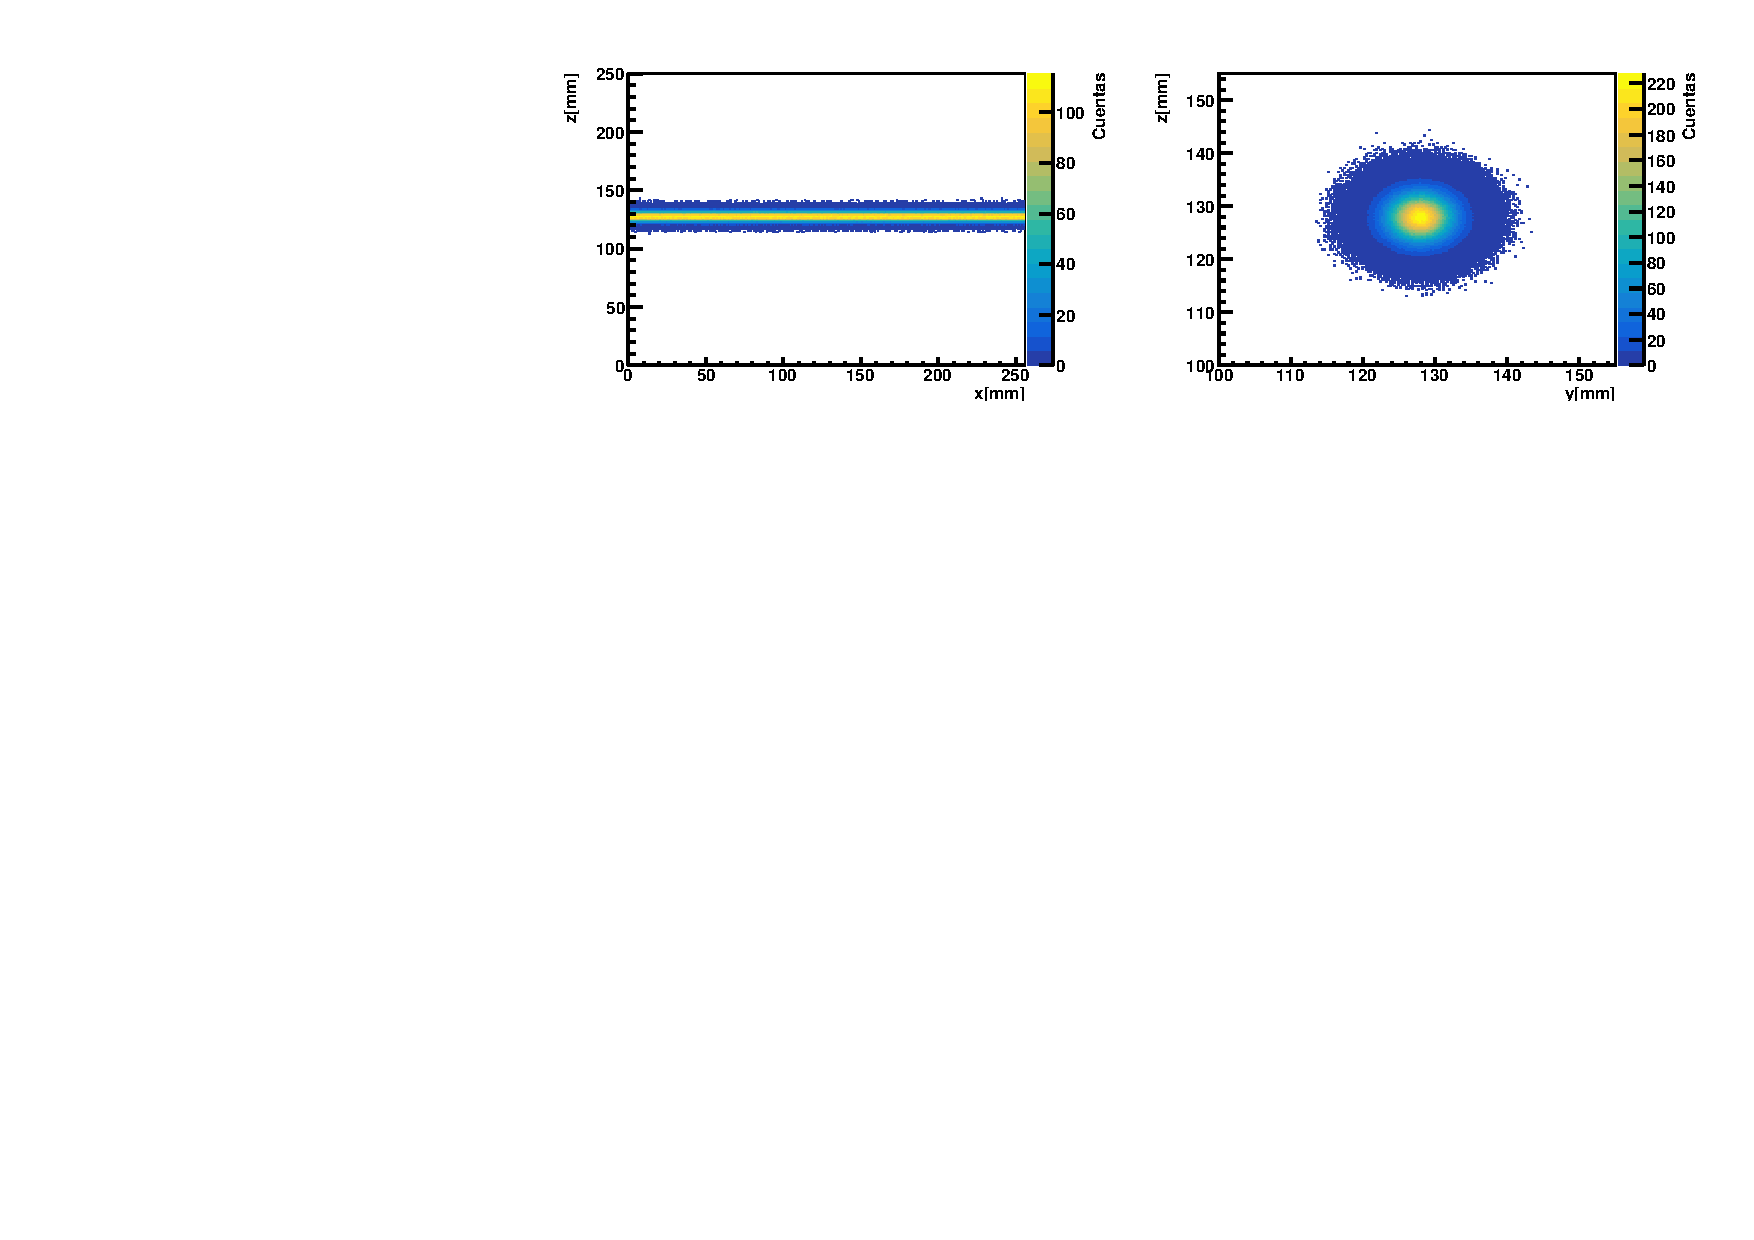
\includegraphics[width=1\linewidth]{Imagenes/Kinematics/Vertex_Ex0.00_incIdx0.pdf}
        \captionof{figure}{Distribución de los vértices de impactos a lo largo de los ejes.}
        \label{Fig:04-Vertex}
    \end{center}
    
    

    \item Lo siguiente es considerar es la cinemática. Una vez elegida la $E_{ex}$ y el punto de interacción, lo que tenemos que hacer es calcular la energía cinética y ángulo en el sistema laboratorio del tritio. Será fundamental tener en cuenta las pérididas de energía del \litioOnce entre la entrada del detector y el vértice de reacción, que realizaremos a través de las tablas de SRIM. Para conocer la dirección de salida del tritio y su energía tendremos que generar un valor aleatorio de la distribución del ángulo en el centro de masas $\theta_{CM}$, que obtendremos usando la distribución de probabilidad dada por de la sección eficaz \cref{Fig:04-seccion_eficaz}. Por otro lado tendremos $\phi_{CM}$ que por definición será igual que $\phi_{lab}$ al estar definido en el plano normal a la transfomación Lorentz, y vendrá dado por una distribución uniforme entre $0$ y $2\pi$. 
    
    
    A través de las ecuaciones del apartado \ref{Subsec:03-cinematica} podremos obtener $T_{lab}$ y la dirección del tritio en el sistema laboratorio. Podemos ver en la \cref{Fig:04-kinSampled0} y \cref{Fig:04-kinSampled2} el valor de la energía cinética del tritio y el ángulo de salida, en un gráfico denominada cinemática de la reacción, en función de la energía de excitación.
    
    \begin{minipage}{0.49\linewidth} \centering
        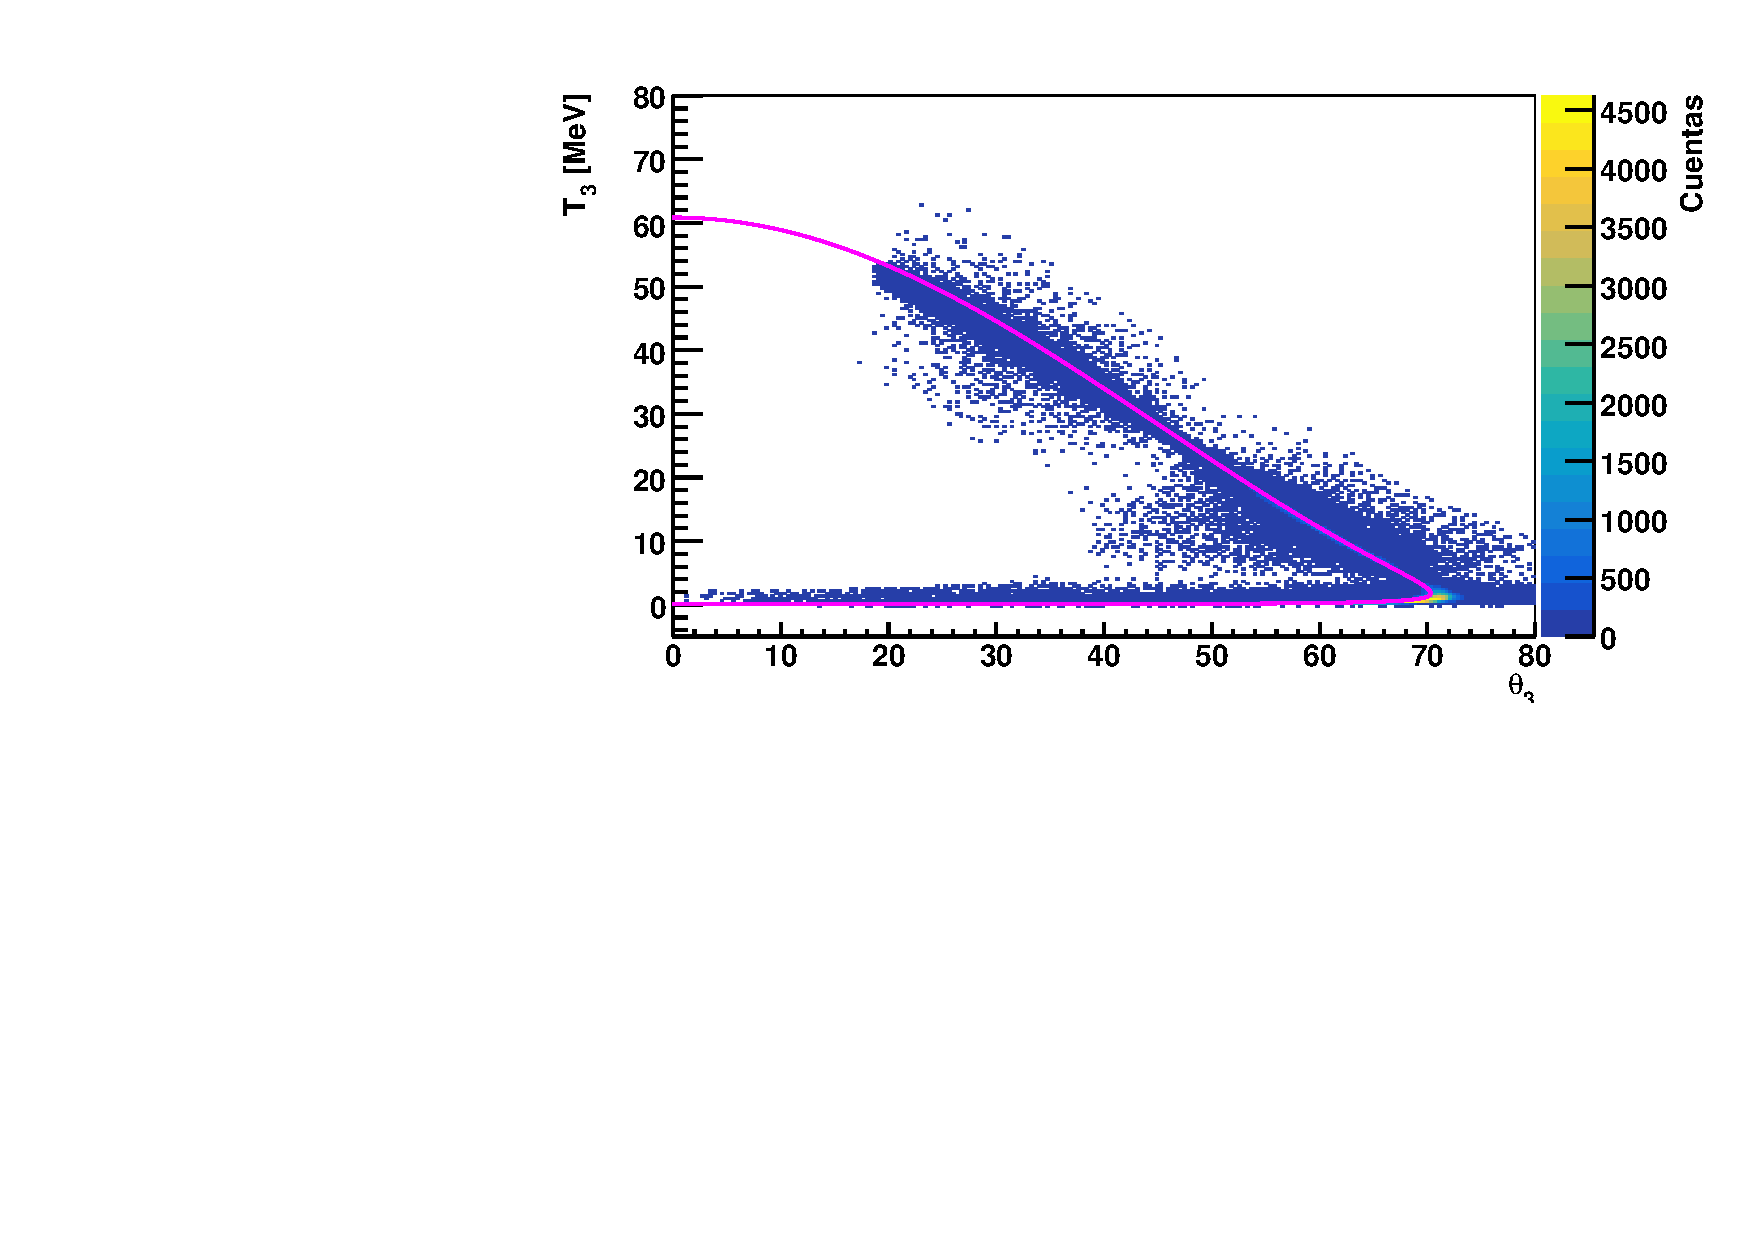
\includegraphics[width=1\linewidth]{Imagenes/Kinematics/KinSampled_Ex0.00_incIdx0.pdf} 
        \captionof{figure}{Cinemática sampleada para $E^*=0.0$ MeV.}

        \label{Fig:04-kinSampled0}
    \end{minipage} \hfill
    \begin{minipage}{0.49\linewidth}
        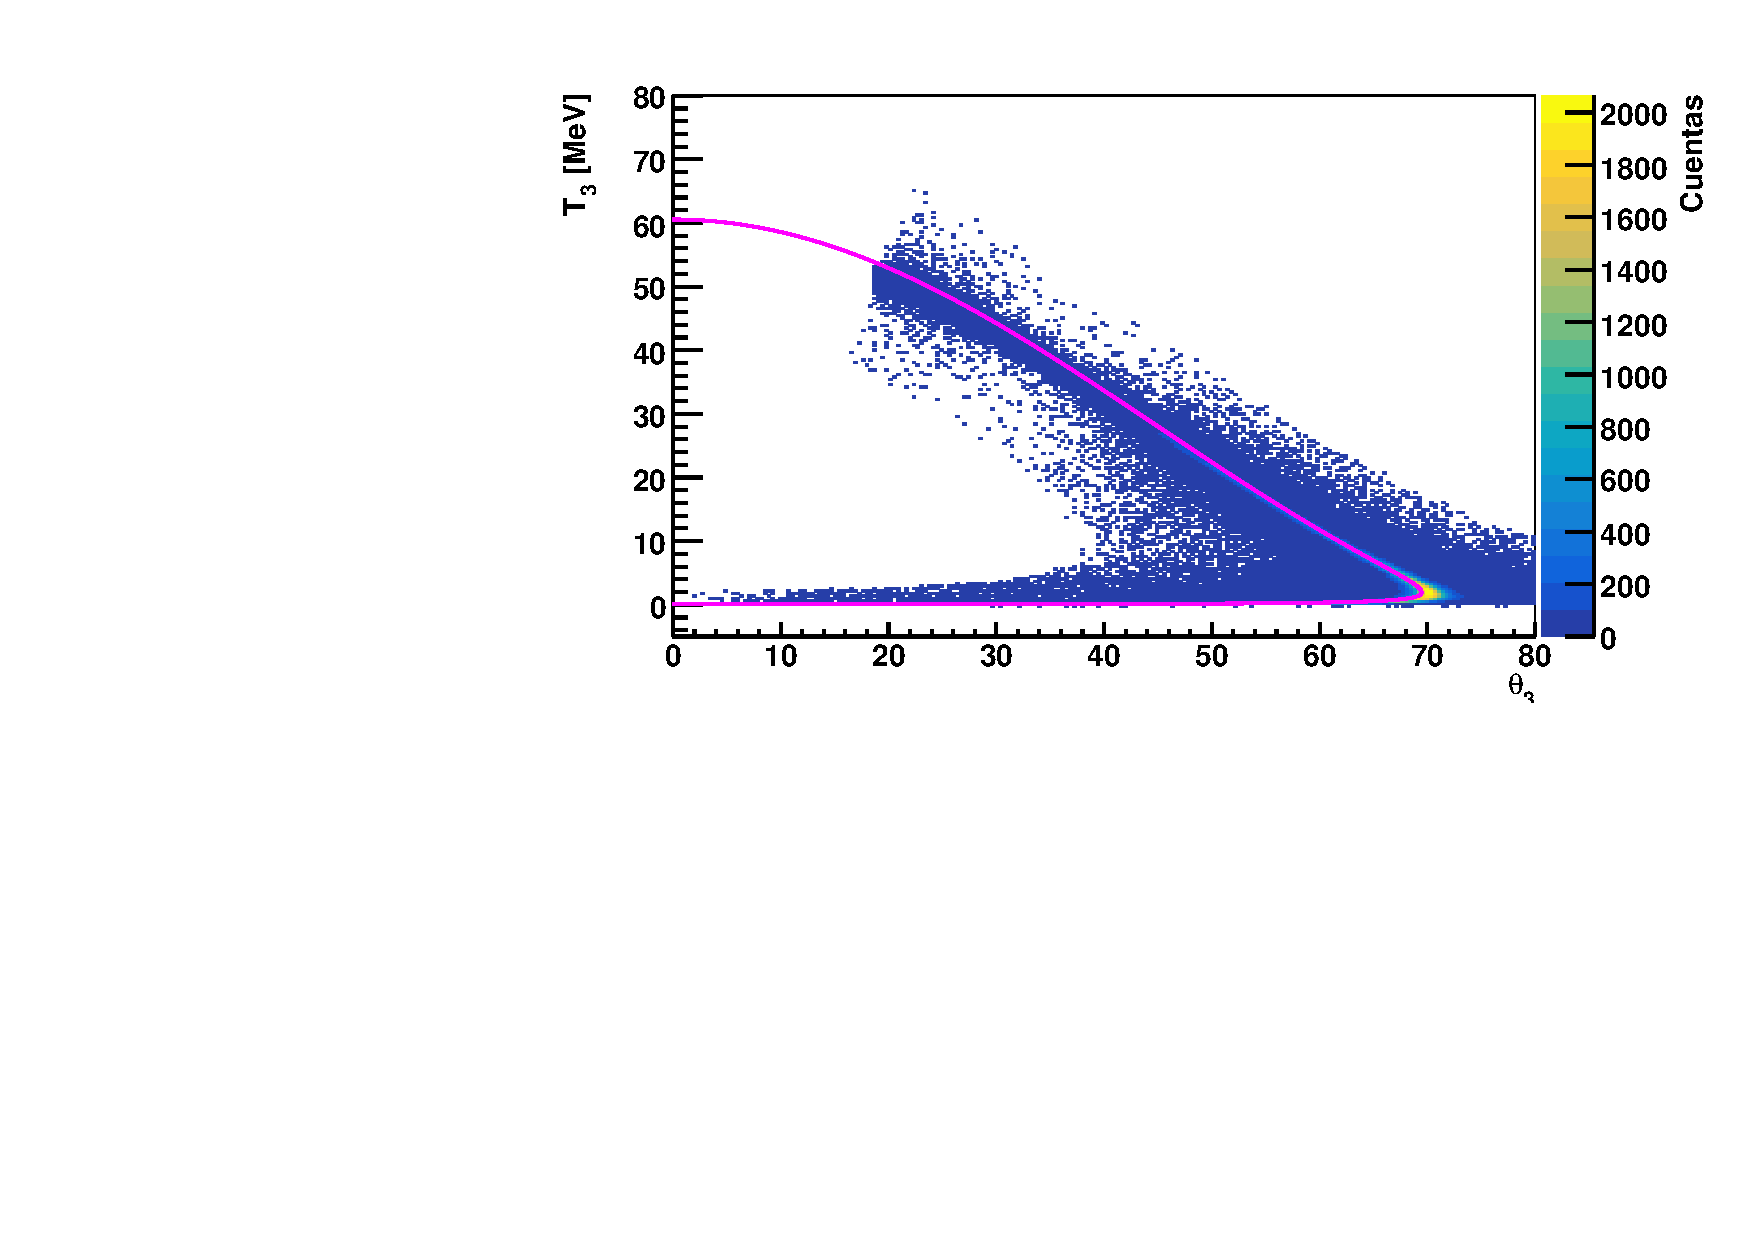
\includegraphics[width=1\linewidth]{Imagenes/Kinematics/KinSampled_Ex0.20_incIdx0.pdf}
        \captionof{figure}{Cinemática sampleada para $E^*=0.2$ MeV.}

        \label{Fig:04-kinSampled2}
    \end{minipage}

    \item También tendremos que tener en cuenta la distribución experimental de los ángulos $\theta_{lab}$, que tal y como ha sido descrito será una normal con FWHM de 1$^{\circ}$. Así pues, tendremos que aplicar esta distribución nada más obtener un $\theta_{lab}$. 

    
    \item Lo siguiente que debemos considerar es si la partícula llega a alguno de los silicios, ubicados según la geometría de \cref{Fig:Geo_Actar}. Para ello trazamos una recta con la dirección del tritio y calculamos la energía con la que llega a dicho silicio. Si la energía es mayor que cero y alcanza a uno de estos su detección es posible. Lógicamente deberemos considerar straggling y pérdidas de energía, por lo que gran parte de los tritios no llegarán a los silicios, puesto que al tener muy baja energía se detienen antes. En la \cref{Fig:04-Impacts} podemos ver la distribución de los tritios que llegan a los silicios, aunque gran parte de estos llegan con una energía mayor de la de \textit{punch-through}.
    

    \begin{center}
        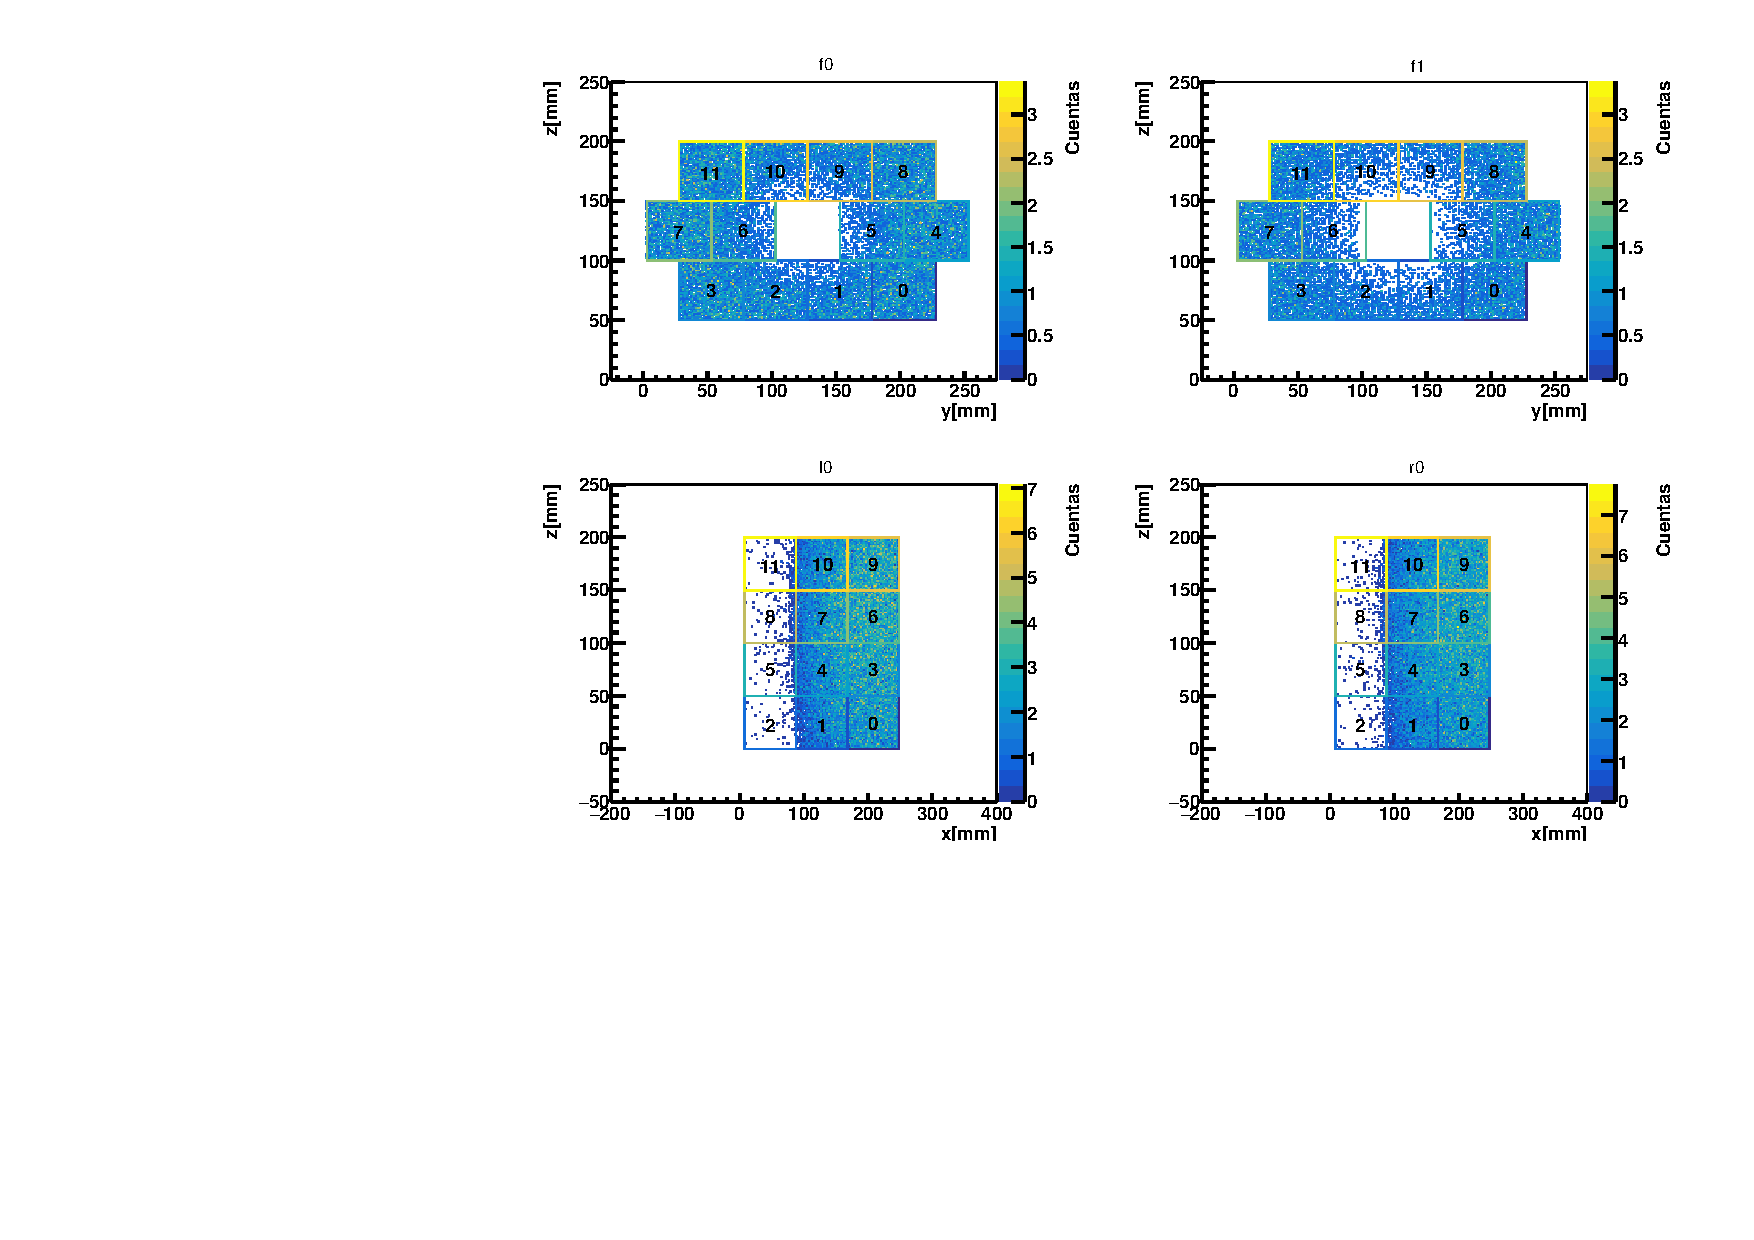
\includegraphics[width=0.95\linewidth]{Imagenes/Impacts/Impacts_Ex0.00_incIdx0.pdf}
        \captionof{figure}{Distribución de los impactos en las 4 layers de silicios. }

        \label{Fig:04-Impacts}
    \end{center}
    

    Se implementa en la cara contraria a la entrada de las partículas una capa de silicios doble, para poder ampliar el número de partículas detectadas y así poder obtener una mejor estadística, sobretodo para aquellas partículas que tengan una alta energía, hasta $\sim 43$ MeV, mientras que solo con f0, l0 y r0 hasta $\sim$ 32 MeV. Para poder afirmar que una partícula ha sido detectada entonces tendrá que frenarse en alguno de los silicios l0, r0, f0 o f1. En aquellos que se frenen en f1 tendremos que considerar la enerǵia depositada también en el silicio f0 así como las energías pérdidas entre ambos silicios.

    La energía depositada la obtendremos como una distribución gaussiana centrada en la energía depositada promedio y $\sigma$ dada por  por \label{Eq:Resolucion_Silicios}. 

    \item Todos los pasos anteriores eran propiamente la simulación, obteniendo todos los valores que podríamos medir el experimento. En este apartado vamos a reconstruir los valores de interés, tal y como se haría en el laboratorio.  A partir de las energías depositadas en los silicios y la posición en la que han sido detectados, podemos determinar inequívocamente la energía del tritio en el punto de interacción. Conociendo la energía cinética y en ángulo $\theta_{\text{Lab}}$ podemos calcular unequívocamente la energía de excitación del $^{10}$Li, ya que esta determina la curva de la cinemática, tal y como podemos ver en la \cref{Fig:04-Kin}. Debido a las diferentes fuentes de incertidumbre implementadas en los anteriores pasos, la distribución de energía de excitación del $^{10}$Li que podamos reconstruir no será una Briet-Wigner, sino una convolución de la distribución de esta con una gaussiana, llamada \textbf{función Voigt}
    \begin{equation}
        V(E;\sigma,\Gamma) \equiv \int_{-\infty}^{\infty} G(E';\sigma) g(E-E';\Gamma) \D E'
    \end{equation}
    siendo $G(E';\sigma)$ la distribución gaussiana y $g(E,\Gamma)$ la distribución Breit-Wigner. En la \cref{Fig:04-Funciones} representamos las distribuciones Voigt, gaussiana y breit-wigner, donde se puede ver la diferencia entre las tres. 

    \begin{figure}[H] \centering
        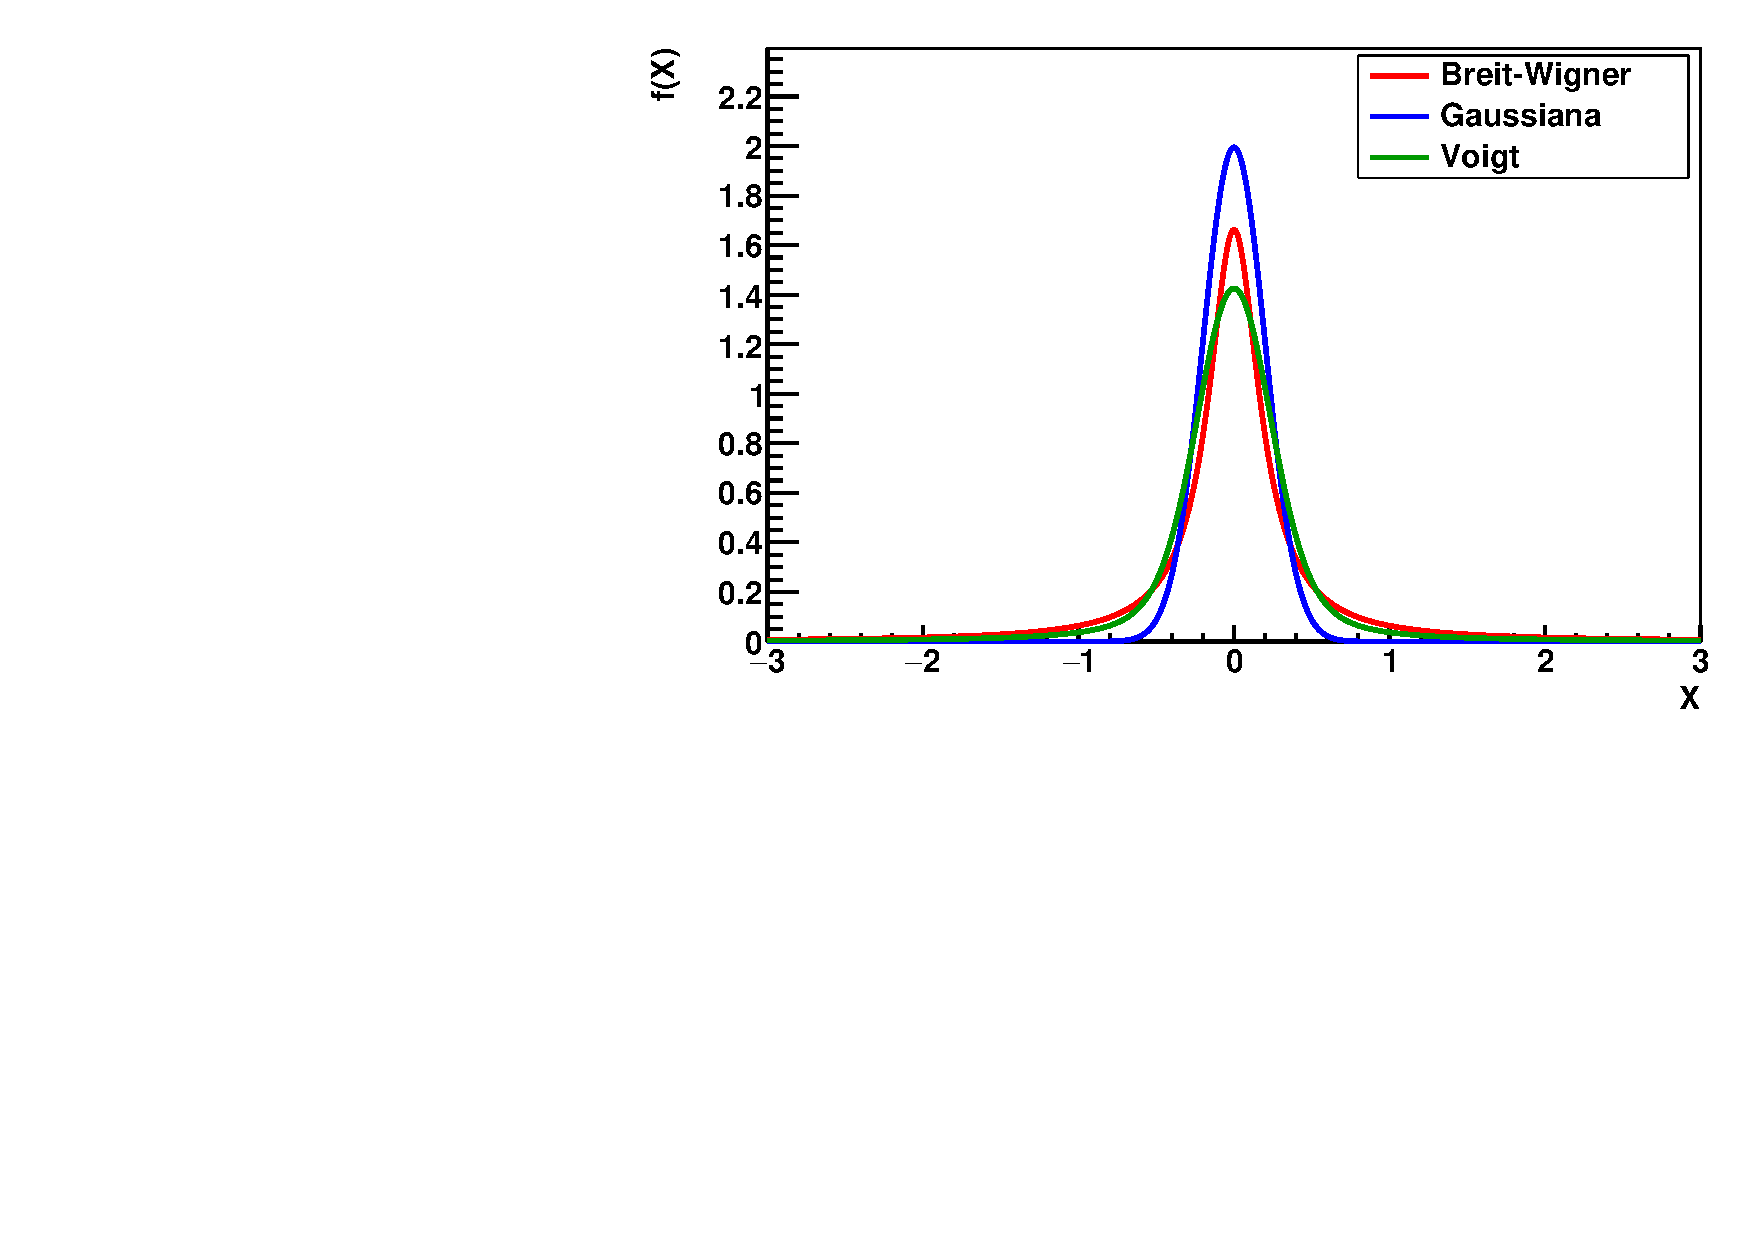
\includegraphics[width=0.7\linewidth]{Imagenes/PlotVoigtGaussBreitWigner.pdf}
        \caption{Distribuciones Breit-Wigner, Gauss y Voigt para $\mu=0$ y $\Gamma = \sigma=0.2$. }
        \label{Fig:04-Funciones}
    \end{figure}
    
    A partir de esta distribución podremos obtener el valor de la energía de excitación, cual es el valor de $\sigma$ dada por todas las diferentes combinaciones, $\Gamma$, la altura y media de la distribución a partir del ajuste que minimice la $\chi^2$. Lógicamente el valor medio de la energía de excitación y la anchura de la resonancia serán los valores que le hayamos introducido (o al menos idealmente). Entre las diferentes combinaciones que encontramos tenemos:
    
    \begin{equation}
        \sigma_{tot}^2 = \sigma_{straggling}^2 + \sigma_{sil}^2 + \sigma_{\theta}^2 
    \end{equation}
    Seleccionando que incertidumbres queremos considerar podremos evaluar que contribución tiene cada una de ellas, y por tanto cual afecta más al experimento, al menos según el algoritmo aquí considerado. Estos resultados se presentan en la siguiente Sección.

\end{enumerate}    
